\label{dad}
\index{Family!dad|(}
\backgroundcolor{c[0]}[HTML]{cccccc}
\backgroundcolor{C[0](10000pt,10000pt)(0.6\columnsep,10000pt)}[HTML]{cccccc}
\backgroundcolor{c[1]}[HTML]{cccccc}
\backgroundcolor{C[1](0.6\columnsep,10000pt)(10000pt,10000pt)}[HTML]{cccccc}

\begin{paracol}{2}
\begin{leftcolumn}
\noindent It's not about the dress.

It's about that whole point in my life. It's about the way home ways. It's about the way I was left to my own devices. Every kid's dream, right?

I had no father. I had the angry, drunken man who lived upstairs. I have the man who woke me in the morning to drive me to school, who clearly showed up at some point during the night. I had this unpredictable animal living in the house that I had to please, and there were no rules for what would or wouldn't please him.

I was left to my own devices and there was always something that I needed to be doing and doing correctly, and I was never sure what it was. Do good in school, sure. Grow up to become an imortant engineer of some kind, sure. The details in between, though, were hazy.

\begin{ally}
The rules are made up and you're always in trouble.
\end{ally}
Or about to be, yes.

\begin{ally}
You know now that he was flailing at life as much as you are now.
\end{ally}
I do.

\begin{ally}
You know now that he was actually in quite a bit of pain.
\end{ally}
Yes.

I also know that he would close out the bar that Julie worked out, drinking the whole time.\index{Family!Julie}

I know that if I went with, I'd spent countless hours meandering between the corner booth in the bar and the Pac-Man and Millipede cabinets up front.

\begin{ally}
The owners of the restaurant would dote on you. They would give you free kitsch from the glass case by the register. Little sticky-backed calenders with tear-off months and pens to draw on the backs of the pages. They'd let you pick out the licorice breathmints from the brass bowl by the register, the ones shaped like chalky pillows. They'd let you play hide-and-seek with Kevin, the other kid being raised in the bar by a drunken father.
\end{ally}
I know that he and Julie had bowling league on Saturdays and I was left home alone.

I know that if I went with, I'd be fed quarters in a steady stream to spend time in the arcade room or on the little toy vending machines.

\begin{ally}
You would buy the little plastic snakes made from links that would let you bend them into squares and cubes. You would drink coke after coke. You would wonder how they managed to oil the lanes so perfectly up to the foul line and no further, and when you saw the machine that did so, you were entranced by its single-minded, track-bound life. You watched him sing Devo's \textbf{I'm Too Sexy} for karaoke, mincing about on the stage and producing gales of laughter in his parody of what he knew of gay culture. You were just starting to think of yourself that way.
\end{ally}
It was a spear through my heart.

\begin{ally}
Tell me about the dress.
\end{ally}
Left to my own devices, I prowled the house.

I stole a beer. I stole some Kahlua. I stole a little bit of brandy, but I hated it. I stole some of his pot. I stole a condom.

\begin{ally}
He was so angry about that. He grilled you and you denied it.
\end{ally}
I realize, later, that the reason he was so angry was because, if I didn't steal it, it would've meant that Julie was cheating on him.

\begin{ally}
Tell me about the dress.
\end{ally}
I stole a paring knife and obsessively sharpened it. I cut at my wrists until, confronted with the realization that I would be asked about it, I stopped and cut on my big toes instead.\index{Mental health!bipolar!depression}

\begin{ally}
You told your friend, Julene. She had no idea what to do, confronted with such information. You were eleven.
\end{ally}
What does one say to being told that your friend is self-harming? I would never tell anyone about self harm again, I promised myself.

\begin{ally}
Tell me about the dress.\index{Gender}
\end{ally}
I tried on Julie's dress. I tried on her teddy. I prowled, naked, through her rack of clothing in the spare room for things to try on. I spent a lot of time naked. I spent a lot of time masturbating. I wondered if I was gay because I tried on her clothing, or I tried on her clothing because I was gay.\index{Family!Julie}

\begin{ally}
You told your friends confidently in third grade that lesbians were just women who wanted to be men and that gay men were just men who wanted to be women.
\end{ally}
Matthew said those things, but he had been dying since birth.

\begin{ally}
Tell me about the dress.
\end{ally}
I tried on Julie's clothes with a mixture of guilt and shame. It was titillating and humiliating. It was transgressive. At some point, I figured that, the ontology of being gay aside, I had better get used to wearing such, as that's just what gay men did.

\begin{ally}
Your anger is cooling down.
\end{ally}
Yeah, it is. I can't tell if it's you shifting it away from my dad and onto the dress, or if it's just getting the words out there that's helping so much.

\begin{ally}
Dig deeper.
\end{ally}
\newpage

\noindent The thing I like to say about my dad is that he didn't really want a son, he wanted a buddy. He wanted someone he could be smart with, or, failing that, be smart at. He wanted someone he could chill with and, at the end of the day, go home.

\begin{ally}
He wanted someone he could drink with. Someone he could take to the bar.
\end{ally}
Yes. He seemed fundamentally uncomfortable with the fact that I was his offspring.

It wasn't an always thing, of course. There were a few times we really connected.

\begin{ally}
Yes.
\end{ally}
One time, we taped up glow in the dark stars on my bedroom ceiling and walls to make my bedroom into a night sky when the lights were out.

\begin{ally}
Yes.
\end{ally}
One time, when driving you to school on a snowy morning, there was an accident far ahead and traffic was stopped on Highway 93, and I had to pee so bad, he had me just step out of the car and pee, blocked off by the door with my back to the car behind me. Traffic started moving then and I had to walk awkwardly to finish peeing before I could hop back inside the moving truck. We laughed. On days we knew we'd be late because of weather, we'd grab french toast sticks from Burger King.

\begin{ally}
Yes.
\end{ally}
One time, we lay on our backs on a beach at Lake Powell and stared up at the real night sky and talked about the satelites that went overhead. We would try to guess, based on how fast they moved, whether we were seeing the same ones again later. He talked of his sisters, Patty and Sue, and how they were doing. He talked of his brother, Joe. He told me Joe was the trouble kid, how he got caught on PCP once and when grandma brought him home from the police station, he missed the door to the house entirely and walked into the door jamb and fell down laughing. Grandma kicked at him, cursing up a storm. He told me about his dad, blowing up an inner tube and floating out into the middle of the pond with a six pack or a bottle of liquor and drinking as he looked up at these very same stars, floating on his back. About how sometimes, his dad would fall asleep out there and grandma would have to throw rocks at him to wake him up the next morning so he could paddle back ashore and get to work.

\begin{ally}
One time, after you switched majors from biochem to music education, you went skiing with him, but had an upset stomach, so you stopped to buy some Alka-Seltzer tablets. You asked what kept them from fizzing until they were dropped in water, and he started to explain about buffers, then cut himself short and said coldly, ``But you won't learn about that, now. I don't expect you really want to know.'' He had you ski alone the rest of the afternoon.
\end{ally}
Yes.

\begin{ally}
One time, you told your best friend in the area, Joseph, that you had rode your bike to the mall, Villa Italia, God rest its weary soul, and bought magic cards. He mentioned that while out with you and your dad, and your dad fell behind a few steps and kicked you. You rode home in silence. Joseph refused to ride with you again.
\end{ally}
Yes.

\begin{ally}
One time, you kissed him on the cheek after he hugged you good night and he laughed in your face. ``You thought I was your mom, didn't you?'' he said, then got up and left the room, shutting the door behind him. You thought, years later, decades later, that he really meant to say, ``You thought I was your parent, didn't you? Best buds don't kiss.'' You never kissed him again, and he never kissed you at all.
\end{ally}
Yes.

\begin{ally}
When teaching you to read with the book Hop on Pop by Dr.~Seuss, he jokingly warned you never to actually hop on him or he'd kick you from one side of the house over the roof to the other, and then back again. Joking, of course, but you were already so terrified of him you believed every word.
\end{ally}
He said the same during our one talk on sex. That if I ever got a girl pregnant and didn't use a condom, he'd do it five times and then leave me on my own to be a dad.

He raised me, but the definition of `raise' here is a very elastic one.

\begin{ally}
Dig deeper.
\end{ally}
\newpage

\noindent The one thing we did together that we both seemed to earnestly enjoy was skiing.

\begin{ally}
There were other things you enjoyed.
\end{ally}
Together?

\begin{ally}
Reading, perhaps?
\end{ally}
He tried to get me to read \emph{Flowers for Algernon}, but I wound up skimming parts, enough to keep him happy when he asked me about them, all while reading the copy of \emph{Mossflower} I'd hidden down the back of the couch. The closest we got was reading \emph{The Dark Tower}.

\begin{ally}
Catch?
\end{ally}
One-sided and short-lived. We played a few times. Then, after telling me to ``get under'' a fly ball, it hit me square on the forehead and he laughed, telling me I was supposed to get my glove up, too. We never played again.

\begin{ally}
The dogs?
\end{ally}
Dad used to punish the dogs by locking then in the basement. If he was really mad, he'd toss then down the stairs by the scruff.

\begin{ally}
School? Math? Computers? Being smart?
\end{ally}
Listen.

You have to understand that there were only two valid emotions for my dad: pride and anger. Being good at computers and math was not something that was enjoyable in its own right. Not for the both of us. The part that we shared there was that we had to have something we could declaim about. Something we could pull out and show that we might be proud of it.

\begin{ally}
So you went skiing, because you both were about the same level at that.
\end{ally}
I bounced, he didn't.

\begin{ally}
That's a factor of your age and size. I don't think you actually bounce all that well.
\end{ally}
Fair.

You're right, though. We went skiing together because that was just sort of the thing we enjoyed --- for different reasons, I'm sure --- and it just so happened that we enjoyed doing it around each other, too.

There would be mishaps, of course. Forgetting boots or poles was a big one. I forgot my poles once and thought I'd be found, dead, in the woods later that day. We wound up renting a pair. From then on, I was determined to learn how to ski without them.

\begin{ally}
It turned out to be fun, at least.
\end{ally}
Yes.

We fell into a habit. Go skiing every other weekend, since that was my time staying with him, from late fall to mid spring. We'd make the drive from the suburbs west of Denver up into the mountains. We'd hit Winter Park, our favorite, or we'd maybe run over to Arapahoe Basin or Loveland Pass.

We'd ski from nine in the morning until about three in the afternoon. We'd grab lunch. Dad would grab `beer-thirty' a little bit after that and let me do a few runs on my own while he chatted up a bartender.

\begin{ally}
You would get the buffalo green chili every lunch, when you wound up at Winter Park. At Loveland, it would be the build-your-own pizzas. It was all so routine.
\end{ally}
It was the most comfortably routine thing that we did together. Not even school could top that.

\begin{ally}
It was, above all, pleasant.
\end{ally}
At times.

\begin{ally}
Yes.
\end{ally}
At times it was stressful. At times it felt like we were going skiing so that my dad could take some time away from home, away from Julie. At times, when Julie came with us, it would be more stressful on the slopes than it was at home.\index{Family!Julie}

And then it fell apart.

\begin{ally}
Yes,
\end{ally}
There's no one time I could point to and say, ``Ah-hah, \emph{this} is when things fell apart.'' There were a few indicators, to be sure, but no one single instance.

There was only that last ski trip to Steamboat.

\begin{ally}
When?
\end{ally}
My birthday.

\begin{ally}
Which?
\end{ally}
I don't even remember. Middle school? Freshman year of high school?

\begin{ally}
Had life started yet?
\end{ally}
It must have. It must have been high school, then. It must have been spring break. It must have been, because I could drive, then. Dad made me take my turn driving his new truck while he sat in the passenger seat and drank glumly. Tecate after Tecate. Julie sat in the back and stayed quiet. Even then the cracks were showing in their relationship.

\begin{ally}
It started snowing on the drive.
\end{ally}
Yes.

\begin{ally}
You drove a fraction of an inch too close to the shoulder, your right wheel veered from the dark tracks plowed through the thin layer of snow by the car in front of you. He shouted, ``Pull over at the next exit, if you're going to drive like that. Snow could cause too much drag on the tires and drag us off the road.''
\end{ally}
Yes.

\begin{ally}
He was drunk and in pain. His shoulder again. He yelled at Julie. Told you both to let him drive in silence.\index{Family!Julie}
\end{ally}
Yes.

\begin{ally}
When you got to the condo that you'd rented. He took four or five advil with a Corona, apologized sullenly, and went to go lay down.
\end{ally}
I don't remember any of the rest of the trip. All I remember is that we watched \emph{Fellowship of the Ring} and that, at one point on the drive back, I asked a question about angular momentum.

\begin{ally}
You wanted to promise him, visibly, that you were still smart. You wanted to appeal to him in a way that you knew he'd take well.
\end{ally}
I wanted him to be okay with me.

\begin{ally}
Dig deeper.
\end{ally}
\newpage
\end{leftcolumn}
\end{paracol}

\begin{paracol}{2}
\begin{leftcolumn}

\noindent If life started in high school, if that was birth, then running away was conception.

\begin{ally}
It was the first sign you gave that you might have a claim of ownership over yourself.
\end{ally}
Is it alright if I include something I wrote about it a long time ago?

\begin{ally}
Maybe.
\end{ally}
Will you feel left out?

\begin{ally}
Maybe. Will you?
\end{ally}
I guess.
\newpage
\null
\thispagestyle{empty}
\newpage
\end{leftcolumn}
\end{paracol}

\index{Family!dad!running away|(}
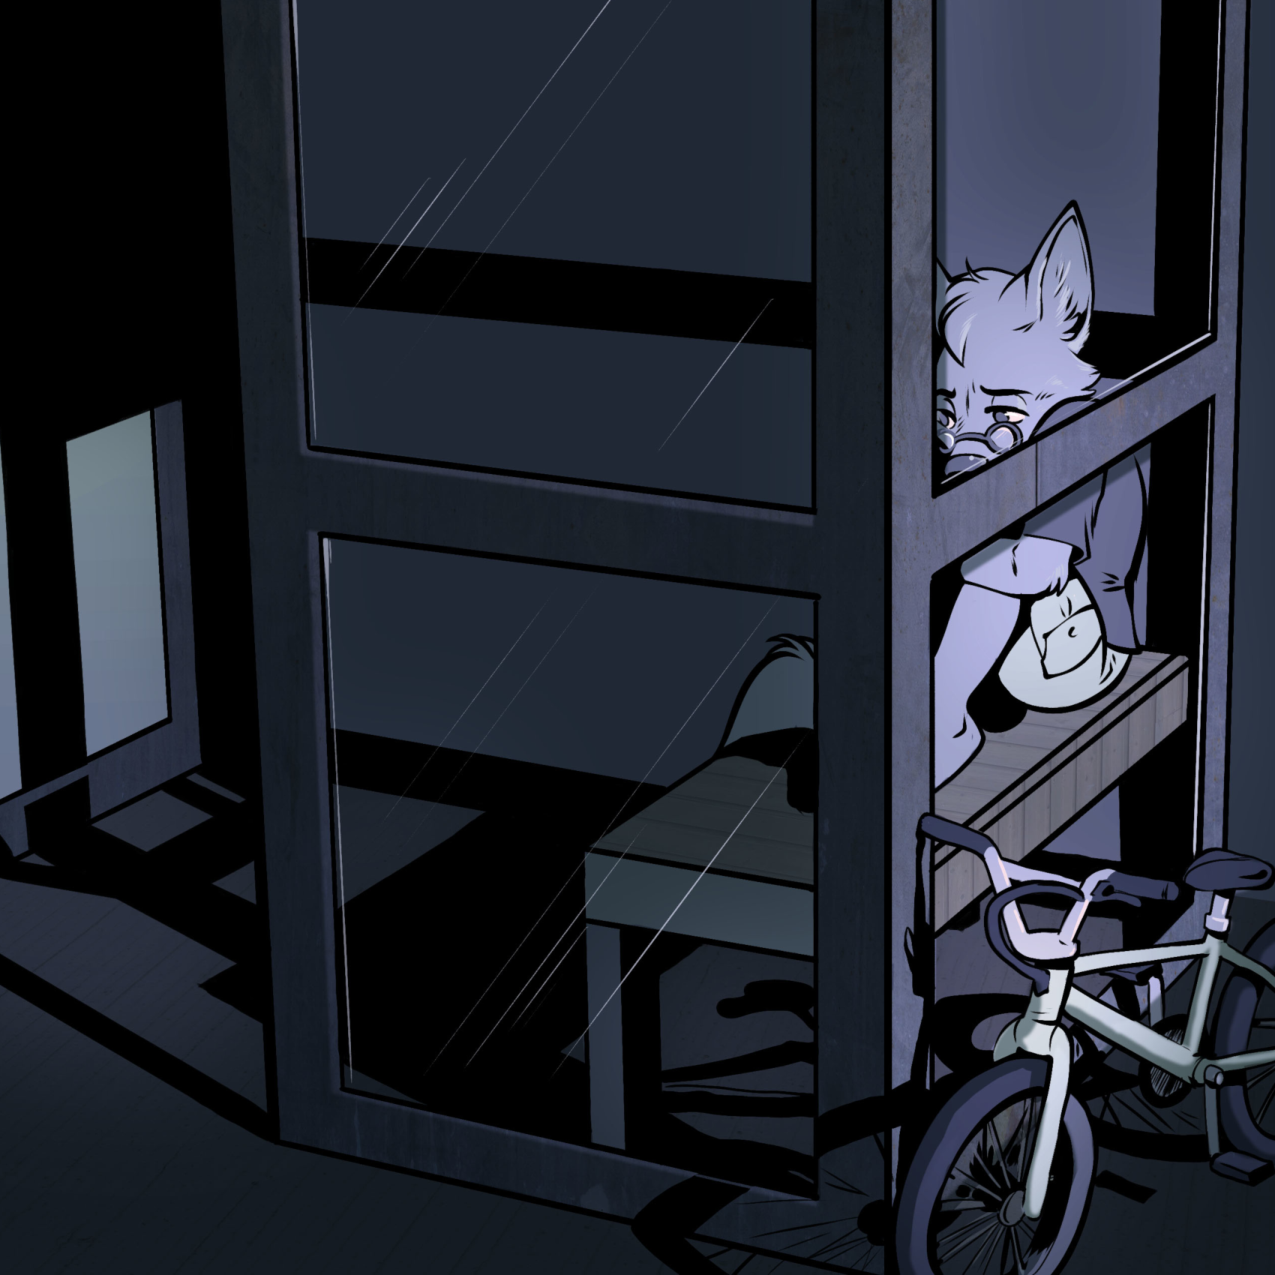
\includepdf{assets/static/grey--running-away-big--makyo.pdf}

\begin{paracol}{2}
  \begin{rightcolumn*}
    \begin{flushright}
      \index{Journal entries}
\emph{June 10, 2015}
\end{flushright}
\end{rightcolumn*}
\begin{leftcolumn}
\noindent I think we all have a lot of formative moments in our lives. For me, it was stuff like coming out, the realization of my own mortality, the suicide attempt, and so on. I think that they tend to fall into two basic categories: those which affect us consciously, which we think about from day to day, with enough frequency to say `often'; and those which affect us more subconsciously, where we can go years or decades without really thinking about them, and yet they still inform so many of your actions.

Running away spent a lot of time in the subconscious camp, quietly informing several aspects of how I viewed myself and how I viewed the world around me. It was only recently, in the last year or so, that it's come to the forefront, thanks largely to recent discussions with friends, family, and therapists. It's only through that process that I've come to realize just how formative an event it really was.

In 1997, at eleven years old, I switched from living with my mom full time to living with my dad full time. My parents had divorced at some point early in my childhood, when I was too young to remember, and I grew up knowing nothing else.

The switch was part of a way to make sure that I grew up to be a balanced person. Having spent so much of my childhood in my mom's household, it was time for me to spend more time with my dad than the schedule that we had maintained until then, Wednesday nights and every other weekend. The move was set for the time when I would be switching schools, anyway -- I had just left fifth grade, and that was the time when middle school started in Boulder county.

I remember feeling a mix of excitement and apprehension as the date neared for the switch. On the one hand, it was exciting to be able to spend more time with my dad, who had always been keen on doing things with me that were fun. We'd go skiing, boating, spend a day trying to make the best paper airplanes, learn how to use the computer. On the other, though, I was apprehensive that I would be spending more time with my dad, who had always been somewhat distant, spending much of his time at the bar where my stepmother worked as a bartender, caring more about the grades that I brought home than my experience in school. In some senses, we were in line with each other and our expectations of what a parent-child relationship should be, and in others, we found ourselves at odds.

Even so, things wound up working out alright for sixth grade. I moved in with my dad, and moved to a new school. I had to spend one more year in elementary school, as Jefferson county didn't start junior high until seventh grade, but it served me well. I wound up in a `gifted and talented' program at the school due to how well I did at my previous school, and found the work to be both more engaging and more intense. My grades started to drop, I started to get bouts of depression and anxiety. At one point, I forged my parents' signatures on my \emph{Friday Folder}, which was supposed to be a weekly communication between my parents and my teacher, leading to a few weeks of being in trouble with both my dad and my mom.

Even so, although I was beginning to struggle for the first time in my life, I did my best to please my dad and maintain the enjoyable, if enigmatic, relationship that we had had up until then. I missed my mom, to be sure, having spent so much of my life until then living primarily with her, but I still felt like I could do well enough and excel in school living with my dad.

\begin{ally}
There is much to talk about.
\end{ally}
Should I stop?

\begin{ally}
No, carry on for now.
\end{ally}
I don't remember much about my summer between sixth and seventh grades, other than I had almost certainly gone back to the summer camp that I had gone to every summer before. I remember that this was the first time I started really enjoying writing. After leaving school for the summer, a friend and I had exchanged addresses and promised to write each other a letter over the summer. I don't remember if we actually did, but those drafts of letters turned into my first attempt at journalling, which would lead me to writing stuff like this -- putting my introspection down in words.

In the fall of 1998, I began seventh grade at junior high, one of those transitions where students go from being the oldest kids in school to the youngest. I figured that school would be similar, that it would be as though class had picked up where it had left off.

It didn't.

Junior high and middle school is when they start introducing separate teachers for separate subjects, rather than a single teacher for core curriculum and separate teachers only for specialized subjects such as art, music, and physical education. This threw me for a loop, at first, and I wasn't really sure why until I started digging back into my past over the last few years. What had started happening as puberty continued to roar through me is that depressive and anxious tendencies really started to take root. I would start fearing math class, rather than the subject of math with a familiar teacher, start worrying about the fact that band was mixed-grade and I would be pitted against eighth graders.

As a pre-teen, I had no idea what anxiety, panic, and depression were. I thought I was going crazy. My journals at the time were filled with fretting that I was having `psychotic episodes' and wondering when these increasingly common attacks would become the new normal and coherent thought the brief rays of sunshine.

At the same time, I remember life getting harder for my dad. Things were happening at work -- bad things -- and while I can't remember if it was that I had become more receptive to this or there had been actual changes, the perceived shift in my dad's mood started to wear on me. Over the summer, he had announced that I was grown-up enough to stay home while he went to the bar for the evening. I'd get home at four or so, and dad would get home at nine or ten at night, having sussed out many of his problems of the day at work. I'd be in bed, or maybe we'd watch Deep Space Nine, and then we'd both go to bed.

\begin{ally}
Do you remember it being this way?
\end{ally}
I don't. Or maybe I do, but the time since when I wrote this has colored my interpretation of it.

\begin{ally}
You sound upset, now. Back when you wrote this, you just sounded weary.
\end{ally}
I suppose I was. I was weary in general, then. I was writing this from a tired, point of view. I was the caryatid. I was tired.

\begin{ally}
You are still.
\end{ally}
I've learned to bear the load a little better.

In junior high, report cards came quarterly. My first one came sometime in October. It was not good.

My dad had become increasingly harsh on the topic of grades over the previous few weeks. Parent teacher conferences had not gone well at all, with my math teacher having particularly harsh things to say about me. I don't even remember on what day of the week this happened, though I want to say Thursday. Dad came home for long enough to make us both dinner before he would head out to the bar. Although neither of us mentioned the fact that my poor grades were in my backpack, he must've known what the date had signified, as, before he left, he said something to the effect of, ``When I get back home from seeing Julie, you'll show me your report card.''

I didn't know what to do. Kill myself? I'd tried half-heartedly in the past. I collected the knife I'd stolen and kept in my desk. It was too dull. I had found a mirror from a makeup compact some days before, and I broke the glass, thinking I could use a piece of that instead, but couldn't manage to get any of the shards of glass actually out of the compact, and as time drew on, I felt less and less like actually dying, as opposed to simply ceasing to be.
\newpage

\begin{ally}
Hold on.
\end{ally}
Yes?

\begin{ally}
Let's take a step back.
\end{ally}
Okay.

\begin{ally}
You're about to mix the clinical with the reality.
\end{ally}
I know. You know that. We wrote this story.

\begin{ally}
Yes.
\end{ally}
Are you having doubts as to posting it?

\begin{ally}
Yes. And here is where you start mixing the clinical with the experiential.
\end{ally}
There is one story, but there are two ways to tell it.

\begin{ally}
Can we retell it?
\end{ally}
The whole thing?

\begin{ally}
No.~You don't have to go back and change what you wrote before, at least not the preceding paragraphs. But we need to make this ours now.
\end{ally}
Is the rest not good?

\begin{ally}
It's all perfectly serviceable. It's all perfectly you-in-2015.
\end{ally}
That it is. I wasn't quite so heavy with the lilac scent on my words in those days.

\begin{ally}
It still gets a little purple.
\end{ally}
I guess.

\begin{ally}
Let's cut a deal, then.
\end{ally}
Oh? You want to edit it?

\begin{ally}
You want to edit it. You want to make it more relevant. You want to make it more 2019. You want to make it fit. You want to understand, not just regurgitate.
\end{ally}
Okay, fair.

\begin{ally}
Let me talk about the clinical side. You go back to the other version of the story.
\end{ally}
Okay.

\begin{ally}
What was happening at this point, is that you were having an honest to goodness panic attack. You were entering a fugue state.\index{Mental health!anxiety}
\end{ally}
I froze for several minutes, probably about an hour, sitting on my bed and holding a broken mirror in my hands. All thoughts had left me, and all I could think about was not being. Not being here, not being at all.

Having decided not to kill myself, I put on a hoodie, went up stairs and emptied the quarter jar of quarters, left the broken mirror on the counter, and grabbed my bike. I had no idea what I would do, where I would go. I just knew that I needed out of there. That place wasn't a place I could be.

Still in a trance, I made my way to what I assumed would be a safe space to hide out for a while, long enough for my dad to not be out looking for me. I don't know why that was something I was thinking of, but it was. I rode my bike to the nearby Wal-Mart, and hid behind it, where the semi trailers were parked. I hid between two storage containers in the back, the stars invisible to me due to the bright lights of the parking lot, and yet the shadows were such that I remained in total darkness.

\begin{ally}
You needed to get away. You needed to not be there. You didn't have the language to explain panic, and you didn't understand the importance of escape.
\end{ally}
Yeah. How could I have? No one had thought to teach me.

\begin{ally}
You had boundaries for what you felt were healthy means of interaction, and no means to communicate when they had been crossed. You had been slogging through anxiety with no way to explain to yourself or others what anxiety was, and you had crossed the point where you could continue to exist in that state.
\end{ally}
The only solution was escape. Escaping into an internal world had worked until my dad demanded to see the report card, and escape by death hadn't panned out. The only route left to me was literally escaping the situation.

As the night wore on and the clock struck nine, I realized that I couldn't stay behind the Wal-Mart forever. I'd need some place to go. With only my bike, my hoodie, and five dollars in quarters, I biked the four miles from where I had been camped to the nearest bus station serving the route that would take me back to Boulder. I had no plans beyond getting to Boulder, other than I figured I could be homeless there in relative safety.

\begin{ally}
That's where you spent the coldest night of your life.
\end{ally}
The last bus to Boulder had already left, and so I was left on my own from about eleven that night until nearly six in the morning. I slept off and on on the bench in the bus-stop shelter. I hadn't brought my bike lock with me, so I kept my bike leaning against the bench where I was dozing. I eventually got too paranoid and tied the sleeve of my hoodie around the top bar of the bike while I huddled deep within the relatively thin cotton of the jacket, no protection against the cold of the Colorado night.

\begin{ally}
At some point during the night, your anxiety abated enough to let you get some more perspective on the situation, and you started to think in terms of what you would do.
\end{ally}
I would take the bus to Boulder, get off near the then-open Crossroads Mall, and see if I could get something to eat.

\begin{ally}
You never quite made it back to baseline in terms of anxiety, however. You were riding on a high, the fugue state constantly re-conquering you and leaving you paralyzed for hours at a time.
\end{ally}
The bus was warm. It had eaten \$3.50 of my total of \$5, but it was totally worth it. I fell asleep in the back seat within minutes of getting on, and was only awoken when the bus reached the end of the line and the kindly driver (who surely knew what was up) shook me awake and helped me onto my bike.

For lack of anything better to do, I rode my bike from the Walnut Street Station to my old elementary school. School wouldn't be starting for another half hour or so, so I camped out in a playground near by, affectionately known as Rock Park. I sat atop the sculpture-\emph{cum}-playground that made up the park's central feature and watched elementary schoolers trudge toward their classes.

\begin{ally}
With a bit of rest under your belt and once more in familiar territory--
\end{ally}
Literally three-quarters of a mile from my mom's house, at the time.

\begin{ally}
--you were starting to come out of your state of panic.
\end{ally}
I was left with the dilemma of basically being a fugitive. I couldn't go to my mom's house, and I could never return to my dad's. I was no longer anxious -- my brain couldn't hold that anymore -- I was simply tired and sad.

Without anywhere to go or anything to do, I made my way back up to my original goal of Crossroads and puttered around the mall for a bit. My \$1.50 wouldn't buy me anything, so I just strolled around the bookstore for a while, always a favorite spot of mine. As I headed back out to where I'd left my bike in front of the entrance, I was startled by a red Honda Civic pulling up directly in front of me. My mom had found me. She admitted immediately that she had been canvasing the bookstores in town looking for me.\index{Family!mom}

\begin{ally}
Even in your current state, you were a total dork.
\end{ally}
The rest of that day and the next were a blur of crying. I was crying. My mom was crying.

\begin{ally}
Your dad may have been crying,
\end{ally}
Maybe, but it wasn't the type of thing I saw or heard from him. Mostly, he was angry.

I remember heated phone calls back and forth several times throughout the next few days. He had found my journal and accused me, ``If you feel like you're going crazy, maybe we should put you in the hospital. Is that what you want from us?''

I couldn't answer.

\begin{ally}
Might've done you some good. Gotten you some help.
\end{ally}
``I'm throwing out a bunch of your stuff, since you don't care about your place here.''

No answer.

\begin{ally}
Stuff. Gifts. Clothing. Toys. Things piled high to, as you felt, buy your loyalty.
\end{ally}
``What's with the broken mirror?''

No answer.

\begin{ally}
You couldn't tell him about the numinous aspect of it that drives that imagery in so many trashy teenage poetry notebooks, about how it came crashing down over you like a wave. And you \textbf{definitely} couldn't tell him about wanting to use it to kill yourself.
\end{ally}
``What is it you want from me?''

\begin{ally}
What \textbf{did} you want from him?
\end{ally}
I struggled for a way to put into words the anxiety, panic, and depression that had slowly taken over my life from the moment puberty had hit, exacerbated by the fact that I was living in a place where I felt distinctly unwelcome. I think I wound up mumbling something about the fact that, with my dad gone all evening at the bar, I had no contact with someone in utter control of my life other than through punishment. Even then, as a child, that only felt partly true.

\begin{ally}
Dig deeper.
\end{ally}
\newpage

\begin{ally}
That was exhausting.
\end{ally}
The old blog post?

\begin{ally}
Yes. Exhausting in the sense that you have to hold three versions of yourself in your head at once. You have to hold in your mind the version of you who, in 1998, had such a large panic attack that he ran away from home. You have to hold in your mind the version of you who, in 2015, was struggling through the early stages of transition, who was finally getting into the meat of things with therapy. And you have to hold me in your mind.
\end{ally}
You have to remember that I'm powered by a small cantaloupe. Holding all three of those in my head at once would be a bit much.

\begin{ally}
One of us was getting squeezed out.
\end{ally}
Did you feel neglected?

\begin{ally}
That's nostalgia\index{Nostalgia}: neglect of the present in favor of the past.
\end{ally}
I suppose it is. I'll refrain from diving into a blog post like that again.

\begin{ally}
You can, just mind your boundaries.
\end{ally}
I will.

\begin{ally}
Tell me about running away.
\end{ally}
Again?

\begin{ally}
You-who-live-in-2019, tell me about running away.
\end{ally}
One of us mentioned before that it was the moment at which I started to assert ownership over myself.

\begin{ally}
We both did.
\end{ally}
I suppose I stand by that, then. Stand by the idea that that was conception to the birth that came in high school.

But it needs some qualifications.

\begin{ally}
Qualify away.
\end{ally}
One qualification that it needs is that, at the moment, just as with so many other forms of conception, it was borne of some baser part of me. It was not some conscious thing. It was not this clean and well-thought-out experience, sleek by design.

It was a release of terror into action. I was blacking out from fear. I was so full of adrenaline that living my life as a vagrant was more acceptable to me than waiting for my dad to come home. It was an act that happened. Not something I did.

\begin{ally}
Some folks try to conceive.
\end{ally}
Fair.

Some folks try and plan out their memoirs.

\begin{ally}
Fair.
\end{ally}
Another qualification that needs to be made is that, while I'm willing to accept this was about the time I started to assert ownership over myself, I don't think it happened while running away. Not that night.

\begin{ally}
When did it happen?
\end{ally}
It happened that morning when I sat atop the rocks of Rock Park. I sat atop the rocks and watched kids walking along the cul-de-sac toward Eisenhower, my old Elementary school.

I watched them walking and thought about how much bigger their backpacks looked than mine did when I was in school.

I watched them and I thought about how big my backpack might get in high school, and realized that I wouldn't find out.

I watched them and I thought about going to knock on the door at my mom's house. It was five blocks away.

\begin{ally}
And then you chose not to.
\end{ally}
Yes.

\begin{ally}
Dig deeper.
\end{ally}
\index{Family!dad!running away|)}
\newpage

\noindent When I was getting ready to leave bConnected, I started struggling with movements. It started as a twitchiness in the hands. It started with a wringing of the fingers. It started with a slight nod of the head. It started in so many tiny ways that I didn't really put together.\index{Mental health!movement disorders}

\begin{quotation}
\noindent Twitching, twitching. Screw lorazepam. Gonna walk the dog instead :D

--- @drab\_makyo August 19, 2012
\end{quotation}

\begin{ally}
Twitch twitch.
\end{ally}
Yeah.

\begin{ally}
And how does this tie in with your dad, again?
\end{ally}
Getting there.

\begin{ally}
I'll be patient.
\end{ally}
Good.

The twitchiness grew worse. It grew to a jerk of the head to the side. It went from the occasional thing to something that hit every second and a half or so. It started impeding my speech. I started stuttering. I lost my balance and had to use a cane for a while.

\begin{ally}
It came and went. Not all of that happened at once.
\end{ally}
When I think back on that time, it's just a smear of time from when I got the offer at Canonical and Further Confusion 2013 a few months later. There are bits of time that stick out as being particularly tic-filled, of course, and bits of time I know I was free of it.

\begin{ally}
You were free of it in Montreal, at your intro sprint.
\end{ally}
Yes, and it came back during UDS in Copenhagen. It came back and it stayed.

\begin{ally}
Did it?
\end{ally}
For our purposes here, yes, it did.

\begin{ally}
`Our'?
\end{ally}
Listen. When your body rebels and tries to shake your brain out through your ears and dislodge your eyes, when your friend dies in a car crash and you only find out about it a week later, when you start a brand new job and fly all the way across the country, then halfway around the world, getting stuck in London along the way, time stops making a whole lot of sense. At some point, I had the tic, and it stayed.

\begin{ally}
Touchy tonight, aren't we?
\end{ally}
You're being as helpful as ever.

\begin{ally}
Not my department.
\end{ally}
At some point during this whole process, Thanksgiving rolled around and I went to visit dad.

\begin{ally}
Oh.
\end{ally}
See?

I emailed him ahead of time, warning him that I was struggling with a transient tic disorder caused --- or at least exacerbated --- by one of my medications. I felt so embarrassed, to be seen by him like that.

\begin{ally}
Like what? Vulnerable?
\end{ally}
Yes. To be seen as week by someone who placed so high a premium on strength.

\begin{ally}
He was hardly a body-builder.
\end{ally}
Well, no. Not physical strength. Moral, perhaps? He certainly prided himself on his composure, and this was me in a state where I was literally unable to maintain my composure.

\begin{ally}
At least you had an excuse for avoiding eye contact.
\end{ally}
It was, oddly, a fairly calm and cozy evening. JD came with. We had some turkey breast. I brought a bottle of bourbon and some homemade cranberry sauce. We talked.

\begin{ally}
It was nice.
\end{ally}
It was. This was at the time in my life where I was learning what the proper amount of `dad' was that I could handle. About three hours. Maybe a little more. Any more than that and we'd both fall back into our old habits. We had much better reunions than we did an ongoing friendship.

\begin{ally}
And you drank, then.\index{Alcohol}
\end{ally}
Yes.

\begin{ally}
You laughed when you knocked the bottle of bourbon off the counter and immediately caught it before it fell to the ground. ``The tic has led to my reflexes getting better,'' you said.
\end{ally}
Dad didn't quite know how to accept me acknowledging my vulnerability.

\begin{ally}
It was nice.
\end{ally}
In a smirking sort of way, I guess. In a \emph{oh wow I'm different now} way. In a \emph{I guess I'm finally starting to grow out of being your son} way.

\begin{ally}
Matthew had died.\index{The Death of Matthew}
\end{ally}
Yes. Matthew had died, and we were doing Thanksgiving together.

\begin{ally}
It was nice.
\end{ally}
It was. He had come to the wedding, so the truth was out, as it were, about JD and I, though he surely had known already. During one of his prior visits to Fort Collins, he had invited me down to grab dinner with him in Lakewood sometime, saying, ``You can bring your\ldots{}ah, you can bring James with you, too.''

\begin{ally}
Tell me about `man'.
\end{ally}
Matthew was dead. Madison was conceived. She would be born soon.

\begin{ally}
Dig deeper.
\end{ally}
\newpage
\index{Gender|(}
\end{leftcolumn}
\begin{rightcolumn*}
  \index{Letters|(}
\emph{October 26, 2014}
\end{rightcolumn*}
\begin{leftcolumn}
\begin{quotation}
\noindent Hey Matt

Been a while since I've heard from you. You guys get all settled in the new house? Need to get together and catch up. Still have that gun for your collection.

Doing well here. Grandma is getting a bit more frail. We are going down for thanksgiving.

Dad

Sent from my BlackBerry 10 smartphone.
\end{quotation}

\begin{ally}
Never one to beat around the bush.
\end{ally}
No indeed.

Three and a half hours later, my reply:

\begin{quotation}
\noindent Hey dad,

Things are going fine at the house, though things are always more expensive than they first seem.  We got the old house rented out, though, and that really helps; the mortgage on that is about \$650, and it's renting for \$1550, so the extra cash really helps with the new place.  Other than finances though, it's going really well.  Loveland's kind of a desert for restaurants and things to do, but we've got enough to keep us occupied at the house.

It's a shame to hear about grandma, but I suppose that's sort of what happens as one gets older.  You'll have to say hi for me, I'll be travelling to Seattle around then.  Things are going okay here, work's going really well and there's lots of travel.  I just got back from Brussels not too long ago and am currently in the Bay Area on the first Actual Vacation I've taken in a while, the rest having been coincidental things with conferences and conventions.  We'll have to meet up sometime for drinks and catching up.

In all, things are going well, though I think I need to be more honest about a big part of my life over the last several years.

In my life as a gay man, I believe I only ever really come out in an explicit manner once.  I was in high school, in my first week of classes, and our counselors came around to our homeroom class to hold some getting-to-know-you exercise.  This consisted of a lot of bored kids and one ``excited'' counselor asking us a series of yes or no questions and having us move to one side of the room for `yes' and the other for `no'.  Being in a progressive town, I didn't expect to be the only kid to answer the question "Will you get married when you grow up?" with no, but sure enough, I was.  I was feeling brave, so, when I was questioned about my response in front of the class, mumbled, "gay marriage is illegal, and I'm gay."

All of the other times I had to come out to family or friends, it was something assumed, or something hinted at.  When I came out to my mom, I did so by leaving a book about gay teens and their stories on her stack of books to read.  Coming out at work at my first job out of college was a matter of being "the one hired by the gay manager", and coming out at my second job was a matter of my relationship with James being included in a portfolio piece --- a data-visualization résumé about my life. When I \emph{officially} came out to you, I did so by inviting you to my wedding to James.  Prior to that, although I assume it was common knowledge, it was unspoken.

Needless to say, I'm not all that good at coming out.

Running away was a turning point for me --- for both of us, really.  I think that we have always been guarded in our communication with each other.  During that time in my life, I felt under intense distress that I couldn't express to you.  Not only did I not have the words, it didn't fit in with what I perceived to be our mode of communication.  I felt stuck, drained, and worthless, and the only path forward to me at the time was escape.

After that incident, however, I shut down even more.  I didn't feel that talking through emotions, feelings, and identity with you was appropriate or allowed.  This was something based off of my perceptions, which were that there are appropriate conversations to have, and that not all conversations fit into this category.  I think --- I hope --- that my perceptions growing up were wrong.  I know that my running away caused a lot of pain, and that's something that I still feel bad about, just as I know that only coming out to you through a wedding invite was not my classiest move, and I feel bad about that as well.

It has been my goal with my friends and partners to have relationships based on the ability to share the emotions and problems that are part and parcel to being a living human being.  Over the last few years, I've worked to open up to my mom as well, letting deliberate honesty take the place of obfuscation and lying through omission about the things that are tough to talk about.  I think that, as my dad, I owe that to you as well.  I want to make up for all the lost conversations that we've never had.  We've made good buddies over the last few decades, and I think it's important that we also make good family.

So what's this about?

I've been having troubles fitting within a masculine role for as long as I can remember.  Early on, this was shown through a disregard for the boyish aspects of childhood: a lack of interest in sports, a fascination with reading the same books Marika (I apologize if I've misspelled her name, I believe that's the first time I've ever written it myself), and a need to keep out of the cliques of other boys in my early school years, except for the crowd of misfits I wound up palling around with, with whom I still keep in touch.

Moving to college, of course, provided all sorts of opportunities to explore.  Although I spent time hanging out in the LGBT student services office and fiddled around with all sorts of different relationships, I still maintained this repressed attitude toward gender.  There is a tendency among gay men to be incredibly misogynistic, and I experienced no shortage of that until I managed to quit that group, about the time I switched into a major that I felt fit me much better.  Working in the music department taught me a lot about how gender roles are cemented within western culture, and in particular, I remember a discussion in which a young woman who had accepted a male part in an operetta was taught how to walk like a man.

Somewhere around then, I understood what feminism was all about.  I realized how everything from wages down to the ways in which we walk are coded toward gender, and I hated it.  I didn't fit this masculine role into which I was born, and there was little to nothing I could do about it.

Gayle Rubin describes gender as the aggregation of "chromosomal sex, hormonal exposure, internal reproductive organs, external genitalia and psychological identifications." Needless to say, there's a lot bound up in the topic, and a whole lot of it made me feel awful.  I spent most of 2012 doing my level best to reject gender in its entirety.  I denied my masculinity as I strived for neutrality and, while I gained quite a bit of insight, I gained little ground in terms of tackling my own problems with my identity.

It's only recently that I've decided to come at this problem of identity and personal friction in an explicit and deliberate fashion.  There are things in my life that make me feel bad - just as there are for everyone - and I've found that it's my job, more than anyone else's, to fix the things in my life that cause me pain.  Identity, after all, is that which we feel about ourselves when under duress.

What this boils down to, really, is that I'm more than just uncomfortable in a masculine role, it causes me intense psychological distress, and so I'm working to fix that.

I've found ways to soothe this friction, however, and, as I mentioned, I'm deliberately pursuing these fronts.  I can do little things, like dress in a less masculine fashion, walk with less swagger, and, to get down to the point, change my name away from something so decidedly masculine.  I'm working on changing my name from Matthew Joseph Scott to Madison Jesse Scott-Clary. It's a way to mitigate this distress, and it's working well from my point of view.  I'm finally being proactive about self-actualization rather than waiting for it to come from the outside, and it's doing me wonders.

I waffle quite a bit on whether or not to adopt the label transgender for myself, but in a lot of ways, it really fits.  `Transgender' is an umbrella term that encompasses most all of gender variance in the human population, and literally just means not identifying with the culturally defined gender roles or categories of male or female as it pertains to one's sex assigned at birth.

Going back to Rubin's definition of gender, it is my psychological identification that is not in line with my biological sex.  I don't really feel ``more like a woman than a man'', so much as I feel decidedly ungendered.  Gender itself is non-binary - there isn't simply an either-or, or a line between two extremes, but a whole realm of experience that exists, unique to each person as an individual.

As far as definitions go, this makes me more ``genderqueer'' or ``genderfluid'', rather than simply ``transgender''.  However, given my tendency to shy away from masculinity, I think it is safe to say that, although I will aways be a man-shape (there's no changing my height, natch), I will be a lot less masculine, and thus to all appearances by society at large more feminine, than I have been in the past.  So while transgender works, I generally describe myself as agender or genderqueer, and use gender-neutral pronouns such as ``they/them/theirs'' to refer to myself.

Big picture, what does this mean?

I've already brought up the name change, and as yet, that's one in a set of very small changes that make up my attempts to alleviate this particular type of distress.  It's these little things --- changing my name, growing my hair out, carefully choosing the clothing that I purchase --- that I've adopted so far as deliberate attempts to make myself feel better

I am, however, still me.  There is nothing above the surface level that is changing.  This has always been me, and will always be me, and there's certainly no changing that.  Little things such as changing my name are ways in which I can better align that sense of self with the ways in which the world perceives me.

These changes allow me to live in a way that makes me content.  I've been searching for a long time for the supposed happiness that comes with being a grown-up, and, like most everyone, decided it's bogus.  However, there really is something to be said for realizing oneself in a way that provides the utmost self-fulfillment that oneself can provide.  What it comes down to is that I feel good here.  I feel better than I have in a long, long time, and I think that my actions speak for themselves: this is who I am.

What does this mean for you?

Dad, I really appreciate all that you've done for me.  I owe so much more to you than I could ever put into words.  So much of the things we did while I was growing up proved formative to who I am today, and there's no expressing the gratitude that I feel for that.  You've given me so much that there's no amount I could give back to repay that.

I understand that the changes that I am making for myself, now that I'm nearing 30, vary in size from minuscule to enormous.  I understand that I am changing some pretty integral parts of myself, some of which you had a say in yourself, such as my name.

What it comes down to is that I'm writing to seek your acceptance.  It needn't be immediate (I'm telling you this in a letter for a reason, take all the time you need in responding), and it needn't necessarily be wholehearted.  However, this is the path that I'm heading down, dad, and I'm determined to do so.  There's years and years and years of thought and emotion bound up inside of these steps I'm taking, and I want you to be aware of them, and, if it's alright by you, for you to be a part of them.

I know that our communication over the years has been rough in places, but lets have this be the opening to a conversation between us about each of us.  I hope to hear back from you soon.

Apologies for so many words, I know I wrote rather a lot.  I'll stop here and leave some links and resources below.  I wish you all the best in work and in life.

Always yours,

Madison Scott-Clary

Some resources:

\begin{enumerate}
  \item A good explanation of neutrois/agender/genderqueer:

    Take everything that you associate with masculinity and put it into a metaphorical yard. Then do the same thing with everything feminine, putting all of that into an adjacent yard. Then, build a low stone wall (not a fence) between them, and put atop this wall everything that you can associate with both genders. Then, imagine that I walked down that wall, picked up a lot of the attributes from that center place, and then the parts from both of the yards that most appealed to me.

  \item A good set of pages on the subject of transgender issues and gender variance as a whole: http://transwhat.org/

  \item A well-written video on non-binary gender, sexuality, and presentation: http://www.youtube.com/watch?v=ibAGYQtk3r4

  \item A friend, who is going through similar changes in their life, wrote a really good analogy on binaries and identities: https://medium.com/@indilatrani/early-birds-and-night-owls-afc59712b0b8

  \item A really good paper on the types of things I've been working through over the past decade or so: http://web.uvic.ca/~ahdevor/Witnessing.pdf
\end{enumerate}
\end{quotation}

\begin{ally}
I'm ashamed to be associated with you.
\end{ally}
Oh come now.

\begin{ally}
2300 words.
\end{ally}
It's not that bad.

\begin{ally}
You have five footnotes
\end{ally}
Okay, maybe it's a little bad.

\begin{ally}
One of them is an academic paper.
\end{ally}
Okay, it's bad.

Remember when I had the accident with the Pathfinder, though?

\begin{ally}
He told you not to talk like a lawyer, that shit happens. I don't think that means write an essay for class.
\end{ally}
Is it your department to experience just how difficult it is to interact with him.

\begin{ally}
No.~It's my department to mirror that back at you.
\end{ally}
Interacting with him was walking a minefield of proclamations. One didn't just discuss a topic. One didn't just feel emotions and have a heart to heart. One learned about something and showed that they knew what they were talking about. I \emph{had} to talk like a lawyer. I \emph{had} to write an essay.

Matthew was dead, and this was me letting him go. Madison was a newborn. Less than two months old. I couldn't not be careful. I was too fragile.

\begin{ally}
What was his reply?
\end{ally}
Four days later.

\begin{quotation}
\noindent Hey Madison

First things first. Congratulation on that vacation. They seem to be hard to come by lately. I know Maurine doesn't consider going to Tucson a vacation any more. We do love San Fran. Maybe a trip this spring. Playing a lot of deadline games this fall and pretty much have been stuck here in the office. Can't bitch. It pays for retirement (whatever that'll be).

Thanks for the letter. I am always glad to get something to read that has some meat to it. Also thanks for sharing your thoughts and feelings. That thing they call life can be a slippery beast and I am always happy when you can feel a little more comfortable walking around. It's funny how easy it is to say that you don't care what people think when deep down your innate reflex is to care.

Anyway, I am truly happy for you. It's your life and it should be as fun and easy as you can make it. Seems thoughtful people tend to beat themselves up while many others can just cruise through life with a grin. I can envy them at times.  It took me a lot of years to learn to just relax and enjoy things. I've had my times when I have gone to see counselors just because I couldn't feel settled down in life. Each time I've learned a little bit about myself that helps slow down the troubles so that the good can be enjoyed. I will always be there if you need me no  matter what your name is or for that matter your gender.

Still looking forward to seeing you Madison. This weekend is a bit of a rush, but we around from then till Thanksgiving. Let me know your address and Maurine and I would love to come up and see the new digs and have some lunch.

Love Dad
\end{quotation}
\index{Letters|)}

\begin{ally}
Dig deeper.
\end{ally}
\newpage

\noindent I went through all this effort to come out to him. It was one of the only times I've come out and had it be 100\% my choice, my words. I could write what I want, explain my feelings.

\begin{ally}
Ish.
\end{ally}
Well, sure. I had to couch it in language catered to him. I had to couch it almost as an apology. But it was my choice to come out, when I could've just hid.

I typed up my letter. I ran it past Robin. I slept on it. I hit send.

\begin{ally}
You hit send and then you put your laptop away and curled up to rest your head on Robin's lap.
\end{ally}
It took a lot out of me. Being vulnerable is exhausting. Being vulnerable around my dad doubly so.

\begin{ally}
It went better than you had hoped.
\end{ally}
Much.

\begin{ally}
And then you met up in person.
\end{ally}
Yes. We met up for dinner in Loveland, and he just couldn't quite do it. JD couldn't come for some reason or another, so it was just me and my dad and Maurine sitting at a table in Door 222.

I went in boy mode. I wasn't quite sure that I was ready to be that vulnerable around him, not enough to be in a skirt and makeup.

\begin{ally}
You came out as ace. You couldn't have been that shy.
\end{ally}
I was also a little drunk. Maybe after a few drinks, I thought maybe a bit more vulnerability might not be such a bad thing.

It was just all too much, though, for someone I saw so infrequently. He couldn't use my name. He couldn't call me Madison.

\begin{ally}
Man. Dude.
\end{ally}
Yeah. That's all I got. I got one `Matt' and an apology, and then the rest of the night, he would only call me `man' or `dude'.

\begin{ally}
Do you think it was intentional?
\end{ally}
Probably not.

\begin{ally}
But it hurt.
\end{ally}
Yes. It's one thing to not be able to remember a name on the spot, or to mess up on pronouns, but it's another to default to specifically gendered terms when your child just came out to you as trans.

I know, I know, they're not \emph{that} gendered. Folks argue that `dude' is gender neutral with some frequency.

\begin{ally}
But still.
\end{ally}
But still.

\begin{ally}
And then you stopped really trying.
\end{ally}
Yeah.

I talked with my therapist not too long ago about what I would tell someone coming out as trans who had a parent who reacted how my dad did, with that same nonchalance, that same uncaring attitude. I said I would tell them to try to make their voice heard up until a point.

``Up until a point?'' she asked. ``Do you think there's a point where you stop trying to make your voice heard?''

``It's less that than it is there's a point where you have to make the cost-benefit analysis and decide whether or not it's worth it to try any harder.''

``That's kind of harsh, don't you think? To say `it's not worth it to continue this relationship with my family member'.''

I shrugged. ``Maybe it is, but at a certain point, it costs more to keep trying that any benefit I would get out of him really listening and understanding.''

\begin{ally}
You cut your losses.
\end{ally}
Yeah. I decided that it was either going to be too much energy or just plain hurt to much to keep trying and to keep failing with him, so I just kinda gave up.

\begin{ally}
You could have kept going.
\end{ally}
Maybe.

\begin{ally}
Maybe he would have come around.
\end{ally}
Maybe.

\begin{ally}
He could have started to see you as his daughter. You could have told him about the HRT, about surgery. You could have told him about drinking and poly and so many other things.
\end{ally}
Maybe. But at this point, it's too many 'maybe's. I'm too tired to deal with something so important with someone I'm not even sure I respect.

\begin{ally}
It's okay not to respect the him that he was around Matthew. What about the him that's around Madison? What about the him that went and sought out therapy? What about the him who said, quietly, ``I was a real asshole. I'm starting to realize that now.''? Is that him not worth loving?
\end{ally}
Maybe I love him.

I'm just not sure I can let my guard down around him enough to respect him.

The him who kicked me, the him who I ran away from, the him who taught me that moods were a thing for cattle and loveplay\ldots{}that him is still too near the surface. I have spent years of my life, hours and hours of therapy, I have spent thousands of dollars trying to unwind what damage he did to me. I resent that. I loathe that I hate who I used to be in part because he made me that way.\index{Family!dad!running away}\index{Gender|)}

Maybe I do love him, I'm just not yet sure that I don't also hate him.
\newpage

\index{Writing!samples!poetry|(}
\index{Dogs}\index{Family!mom}
\begin{verse}[1.01\textwidth]
  There's some duality between sources of meaning,\\
  \vin Between the types of stories we use to back identity.\\
  It's not quite good \& bad or light \& dark,\\
  \vin Though I'm not yet sure just how to define it.

  Dad used to punish the dogs\\
  \vin by locking then in the basement.\\
  If he was really mad,\\
  \vin he'd toss then down there by the scruff.

  Mom moved me \& her dogs to a new house ---\\
  \vin moved us three days early during the divorce.\\
  Her dog punched my ex stepdad in the crotch the night before,\\
  \vin the nut-shot to end all nut-shots, \& our time there.

  Few things make me feel as deeply about life as parenthood,\\
  \vin even if it's just me caring for my dogs.\\
  Some reminders of that are intense enough to be raw, painful,\\
  \vin salt in the wounds of mortality, maybe, or the ache of maternal love.

  The meaning behind the story of me \& my dogs\\
  \vin comes with a story of its own, or maybe several.\\
  It's bound up in stories to come,\\
  \vin \& these stories nest infinitely deep.

  Remembering that \& shaping that,\\
  \vin It's a part of making the meaning in my life.\\
  This isn't better against worse,\\
  \vin it's not mom against dad.

  It's not a dichotomy at all, really,\\
  \vin now that I think about it.\\
  It's something subtler, comfortably complex, a topic of its own.\\
  \vin I guess it's just meaning \& self.
\end{verse}
\index{Writing!samples!poetry|)}

\newpage

\null
\vfill
\begin{ally}
Do you ever worry that maybe he should be forgiven?
\end{ally}
Oh, \emph{constantly}.
\vfill
\newpage
\end{leftcolumn}
\end{paracol}
\resetbackgroundcolor
\index{Family!dad|)}
